\documentclass[english]{template/fitthesispresn.cls}

\projectinfo{
    date=\today,
    title={Červeno-čierny strom},
    title.footer={Červeno-čierny strom},
    subtitle={5. projekt, ITY},
    author.name={Katarína},
    author.surname={Mečiarová}
}

%struktura
\begin{document}
    \frame[plain]{\titlepage}

    \begin{frame}
        \frametitle{Motivace}
        \begin{columns}
            \column{0.4\textwidth}
            \begin{itemize}
                \item \emph{Algoritmy} sú jedným zo \emph{základných prvkov spracovania informácií}
                \\
                \item Čo je to \emph{červeno-čierny strom}?
                \subitem Od vzniku, cez praktické využitie až do končín teórie
            \end{itemize}
            \column{0.6\textwidth}
        \end{columns}
    \end{frame}


    \begin{frame}
        \frametitle{"\ldots the rest is \epmph{history}"}
        \begin{columns}
            \column{0.4\textwidth}
            \begin{itemize}
                \item Kto? \emph{Rudolf Bayer}
                    \subitem symetrický binární B-strom
                \item Leo J. Guibase, Robert Sedgewick
                \item Kedy? \emph{1972}, premenované 1978, \ldots 1993, 1999
                \item Ako? To si rozoberieme na drobné v nasledujúcom slajde ->
            \end{itemize}
            \column{0.6\textwidth}
        \end{columns}
    \end{frame}
    \begin{frame}
        \frametitle{"\ldots the rest is \epmph{history}"}
        \begin{columns}
            \column{0.4\textwidth}

                \emph{1972}
                \emph{1978}
                \emph{1993}
                \emph{1999}
                \item Čo s tým?

            \column{0.6\textwidth}
        \end{columns}
    \end{frame}









    \appendix{}
    \begin{frame}
        \frametitle{Otázky oponenta}
        \begin{itemize}
            \item Pokud je otázek více, lze udělat i~více slajdů.
            \item Tento slajd nechť je příloha, která se nepočítá do celkového počtu slajdů.
            \item Otázku je dobré sem přepsat \emph{verbatim}, ať není pochybnost, jestli nedošlo k nepřesnému parafrázování.
        \end{itemize}
        \bigskip
        %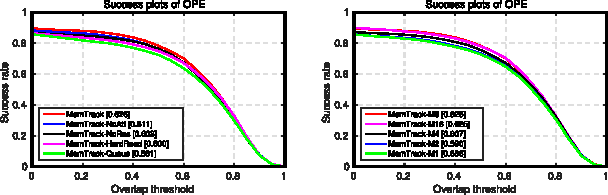
\includegraphics[width=\textwidth]{img/template-ResultsPlot.pdf}
    \end{frame}

\end{document}

